\documentclass[a4paper,twoside]{ctexart}
\usepackage{geometry}
\geometry{margin=1cm,vmargin={0pt,1cm}}
\setlength{\topmargin}{-2cm}
\setlength{\paperheight}{23cm}
\setlength{\paperwidth}{18cm}
\setlength{\textheight}{19.6cm}
\setlength{\textwidth}{15cm}
\usepackage{makecell}
%\usepackage{fancyhdr}
\usepackage{siunitx}
\usepackage{amssymb}
\usepackage{indentfirst}
\setlength{\parindent}{0.5em}

\pagenumbering{arabic} 

% useful packages.
\usepackage{multirow}
\usepackage{caption}
\usepackage{mathrsfs}
\usepackage{amsfonts}
\usepackage{amsmath}
\usepackage{amsthm}
\usepackage{enumerate}
\usepackage{xcolor,graphicx,float,subfigure}
\usepackage{epstopdf}
\usepackage{multicol}
\usepackage{fancyhdr}
\usepackage{layout}
\usepackage{listings}
\usepackage{dsfont}
\lstset{language=Matlab}
\lstset{breaklines}
\lstset{extendedchars=false}
\usepackage[colorlinks,linkcolor=blue]{hyperref}
\usepackage{xcolor}
%\usepackage{cite}
%\usepackage[numbers,sort&compress]{natbib} 
%\setcitestyle{open={},close={}}
%\usepackage{natbibspacing}
%\renewcommand{\refname}{}
\usepackage{anyfontsize}

\usepackage{tikz}
\usetikzlibrary{calc}
\usetikzlibrary{arrows.meta}
\tikzset{
  dot/.style={
    circle, fill=black, inner sep=1pt, outer sep=0pt
  },
  dot label/.style={
    circle, inner sep=0pt, outer sep=1pt
  }
  arrow1/.style = {
    draw = black, thick, -{Latex[length = 4mm, width = 1.5mm]},
  }
}

\newtheorem{theorem}{定理}[section]
\newtheorem{corollary}[theorem]{推论}
\newtheorem{lemma}[theorem]{引理}
\newtheorem{definition}[theorem]{定义}
\newtheorem{proposition}[theorem]{性质}
\newtheorem{example}[theorem]{例子}
\newtheorem{notation}[theorem]{记号}
\newtheorem{algorithm}[theorem]{算法}


\newcommand{\dif}{\mathrm{d}}
\newcommand{\avg}[1]{\left\langle #1 \right\rangle}
\newcommand{\difFrac}[2]{\frac{\dif #1}{\dif #2}}
\newcommand{\pdfFrac}[2]{\frac{\partial #1}{\partial #2}}
\newcommand{\OFL}{\mathrm{OFL}}
\newcommand{\UFL}{\mathrm{UFL}}
\newcommand{\fl}{\mathrm{fl}}
\newcommand{\op}{\odot}
\newcommand{\Eabs}{E_{\mathrm{abs}}}
\newcommand{\Erel}{E_{\mathrm{rel}}}

\newcommand{\Zero}{\hat{0}}
\newcommand{\One}{\hat{1}}
\newcommand{\Int}{\mathrm{int}}
\newcommand{\unitV}{\mathds{1}}

\newcommand{\bmi}{\mathbf{i}}
\newcommand{\bmj}{\mathbf{j}}
\newcommand{\bmn}{\mathbf{n}}

\newcommand{\dist}[2]{\text{dist}\left(#1, #2\right)}
\newcommand{\scientific}[2]{#1 \times 10^{#2}}


%\newcommand{\Dim}{{\mathbf{D}}}
\newcommand{\Dim}{{\scriptsize \textsf{D}}}
\newcommand{\me}{\mathrm{e}}
\newcommand{\mi}{\mathrm{i}}

%\newcommand{\mod}{\mathrm{mod}}
\newcommand{\curve}[1]{\widetilde{#1}}
%\newcommand{\dt}{\delta t}
\newcommand{\dt}{\tau}
\newcommand{\isCovered}{\mathbin{ < \! \! \! \! \cdot }}
%\newcommand{\cIncluded}{\mathbin{ \prec \! \! \! \cdot }}
\newcommand{\coveredBy}{\lhd}
%\newcommand{\regrz}[1]{\mathrm{cl}\left(\mathrm{int}\left(#1\right)\right)}
\newcommand{\regrz}[1]{\mathrm{reg}\left(#1\right)}
%\newcommand{\sgncup}{\ \hat{\cup} \ }
\newcommand{\Span}{\mathrm{span}}
\newcommand{\timeline}[2]{\phi_{t_0}^{#1}\left( #2 \right)}
\newcommand{\timeBP}[1]{\overleftarrow{#1}}
\newcommand{\timeBPA}[1]{\mathring{\overleftarrow{#1}}}
\newcommand{\streak}[2]{\Psi_{t_0}^{#1}\left(#2\right)}
\newcommand{\timelineA}[2]{\mathring{\phi}_{t_0,#2}^{#1}}
\newcommand{\DRLN}[1]{{\cal D}_{\curve{#1}}}
\newcommand{\DRLLN}[1]{{\cal D}_{\overline{#1}}}
\newcommand{\DRLNA}[1]{\mathring{\cal D}_{\curve{#1}}}
%\newcommand{\oplusDR}{\,\overline{\oplus}\,}
\newcommand{\oplusDR}{\,\bar{\oplus}\,}
\newcommand{\qo}{\hat{q}}
\newcommand{\xo}{\hat{x}}
\newcommand{\yo}{\hat{y}}
\newcommand{\closure}[1]{\textrm{cl}\left(#1\right)}
\newcommand{\vertexSequence}[4]{
  \left( #1 \rightarrow #2 \rightarrow #3 \rightarrow #4 \rightarrow #1\right)}

\newcommand{\ppSpace}{\Pi_{<\kappa,\bm{\xi},\bm{\nu}}}
\newcommand{\pnSpace}{\mathbb{P}_{<\kappa}}
\newcommand{\pnSpaceK}[1]{\mathbb{P}_{#1}}

\newcommand{\Pyr}[2]{\textrm{Pyr}_{\cal{#1}}\left(\mathbf{#2}\right)}

%\pagestyle{plain}
\pagestyle{fancy}
\fancyhf{}
\fancyhead[LE,RO]{\textbf{\thepage}}

\makeatletter
\newcommand\sixteen{\@setfontsize\sixteen{17pt}{6}}
\renewcommand{\maketitle}{\bgroup\setlength{\parindent}{0pt}
\begin{flushleft}
\sixteen\bfseries \@title
\end{flushleft}
\textit{\@author}
\egroup}
\makeatother

\CTEXsetup[format={\Large\bfseries}]{section}

\title{井旁二维地质构造剖面精细建模项目文档}
\author{刘骥宇、李泓睿}

\begin{document}
\maketitle

\section{项目背景}

在地球科学研究及资源勘探开发领域,二维地质构造剖面是一种不可或缺的基础
性图件。它通过沿特定方位(通常垂直于区域构造走向或构造轴线)的垂直平面,
系统性地表达地下地质体(如地层、岩体、构造要素)在垂向和侧向上的空间展
布、几何形态、接触关系及岩性配置特征。

二维地质构造剖面在多个关键环节发挥着核心作用:
为理解区域构造格架、应力场演化及构造变形机制提供最直接的几何学约
  束,是建立三维地质模型不可或缺的前期工作与核心验证依据,为复杂地质体
  的空间建模奠定基础;
  在油气、矿产、地热等资源勘探中,是圈定目标储集体(如储层、矿体)、
  刻画其几何形态(空间展布范围、厚度变化趋势)和评估连续性的核心图件,
  直接影响资源储量计算的可靠性和精度,为勘探目标优选与评价提供地质依据;
  作为钻井轨迹设计的“地下导航图”,确保井眼精确穿越目标层位并规避
  风险(如断层带、高压层),可显著降低钻井工程风险,提高钻遇率和工程效
  率。

构建高精度二维构造剖面的核心数据源来自于钻井测井,特别是高分辨率井壁成
像测井(如声、电成像)。这些数据能够沿井孔轨迹获取连续、高精度的岩层产
状信息,包括地层倾角和倾向。

\begin{figure}[htbp]
  \centering
    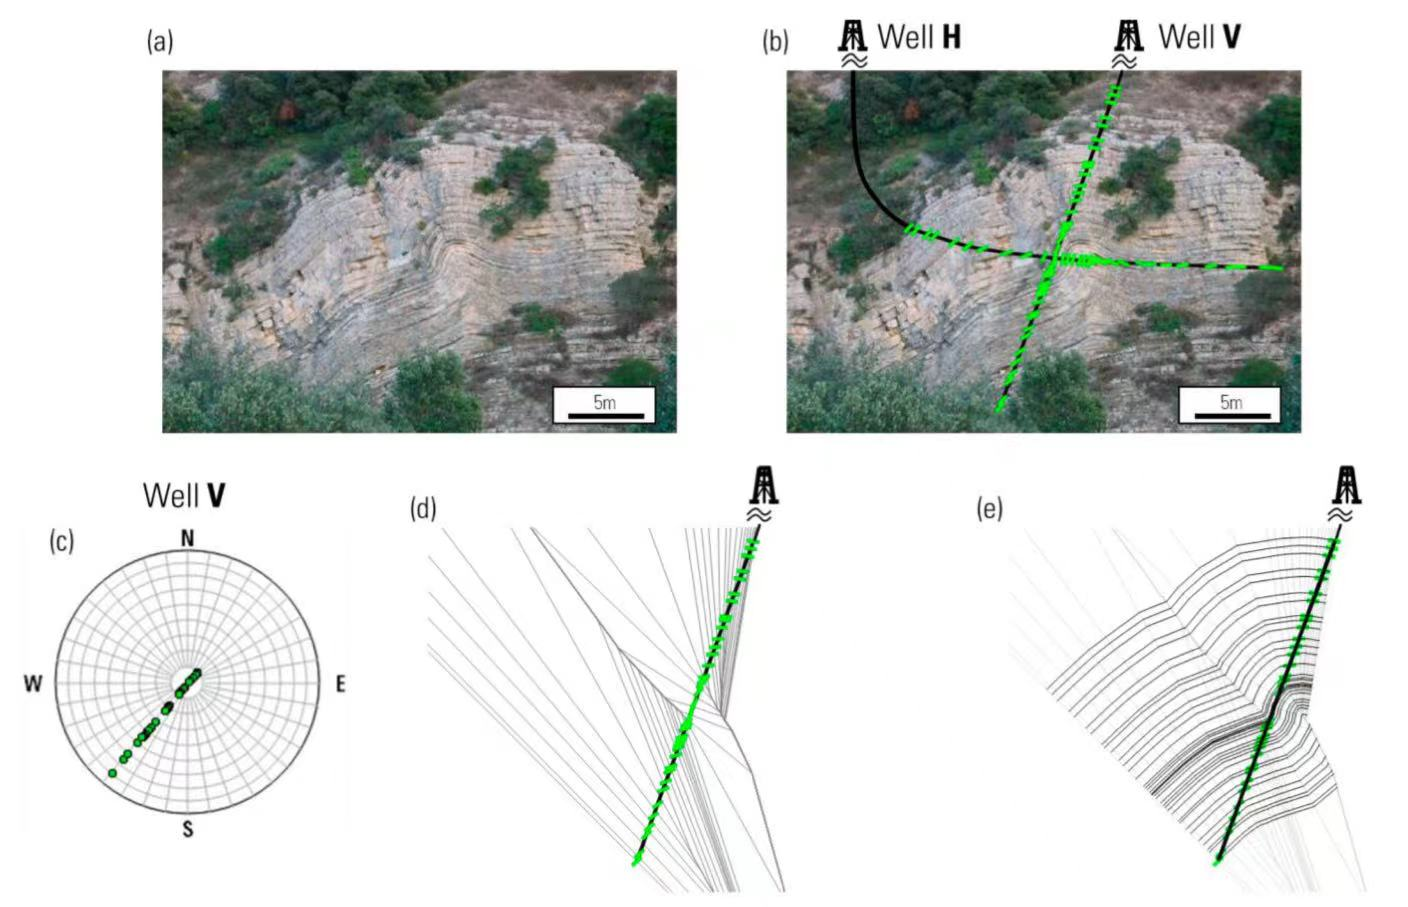
\includegraphics[width=0.65\textwidth]{pic/剖面例图.jpeg}
  \caption{二维地质构造剖面示例,子图(e)为根据井$\mathbf{V}$的钻井数据
    生成的地质构造剖面}
  \label{fig:二维地质构造剖面示例}
\end{figure}

然而,钻井数据本质上是离散的、一维的(沿
井轨迹分布的点或短区间数据),仅能反映井孔局部(厘米至米级尺度)的地质
特征。尤其在挤压或伸展构造区(如褶皱转折端),基
于平行层假设的建模方法因忽略地层厚度变化、岩层旋转等动态特征,导致储层
几何形态误差增大,严重制约复杂构造区的资源评价精度。
因此,核心建模挑战为如何基于井轨迹上有限的离散岩层产状观测点,通过合理
的数学地质算法,在选定的二维剖面上重建地质层面在远
离井孔区域(十米至千米级尺度)的连续、合理且符合地质规律的空间延伸轨迹。

针对上述问题,本项目提出一种基于蛛网算法的新型建模框架,构建符合地质力
学规律的地质模型,为复杂构造区的资源勘探与开发提供高精度地质模型支撑。

\section{预备知识}
\label{sec:Preliminary}

\subsection{地层构造}

地层是指在地球历史某一特定地质时期内形成的、具有显著共同特征(如岩性、
化石组合、沉积构造)或成因(如沉积、火山喷发)的层状岩石或沉积地质体。
它们在空间上呈层状或似层状展布,其垂向叠置序列系统性地记录了该区域地质
演化过程中的沉积环境变迁、构造活动、古生物演化及古气候条件等关键信息。

依据可观察的岩性特征及其组合、地层位置和接触关系,地质学建立了地层年代
表,用于划分和对比全球地质历史的时间框架体系,它以地质年代单位(如:宙
Eon、代 Era、纪 Period、世 Epoch、期 Age)来标定地质时间的绝对或相对间
隔,可用地层年代表表示。
不同地质年代生成的地层构造的特性各不相同,由此会出现地层分层,图
\ref{fig:地层分层剖面} 中各字母分别代表不同地质年代生成的地层构造。 
  \begin{figure}[htbp]
  \centering
    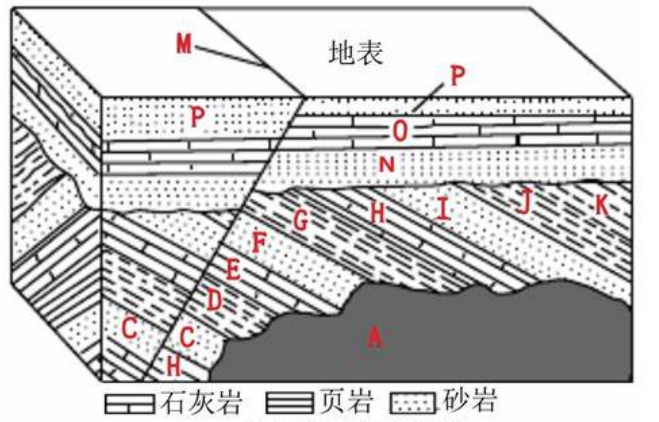
\includegraphics[width=0.6\textwidth]{pic/地层年代剖面.png}
  \caption{地层分层剖面示意图}
  \label{fig:地层分层剖面}
\end{figure}

下面介绍两种主要的地层构造:褶皱构造和断层构造。 

\subsubsection{褶皱构造}
\textbf{褶皱构造}是岩层在构造应力(如挤压)作用下发生的弯曲变形。反映
区域水平挤压作用,常见于造山带,是油气储集的重要构造。基于形态特征分为
以下三类: 
\begin{enumerate}
\item \textbf{背斜(Anticline):}岩层向上拱起,核心部位(褶皱的几何中
  心部位)为老地层。
\item \textbf{向斜(Syncline):}岩层向下弯曲,核心部位为新地层。
\item \textbf{单斜(Monocline):}岩层向单一方向倾斜的平缓弯曲。
\end{enumerate}

 \begin{figure}[htbp]
  \centering
  \subfigure[背斜和向斜构造]{
    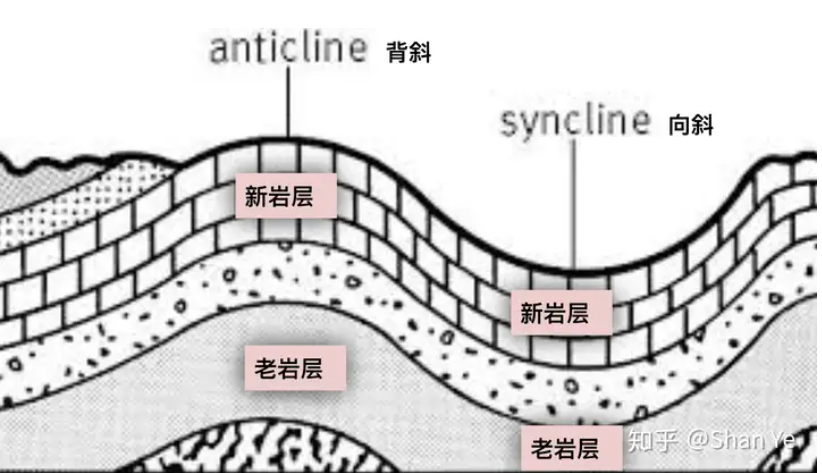
\includegraphics[width=0.35\textwidth]{pic/背斜和向斜.png}
  }
  \hspace{2cm}
  \subfigure[单斜构造]{
    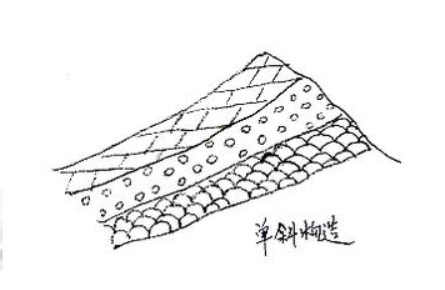
\includegraphics[width=0.35\textwidth]{pic/单斜构造.png}}
  
  \caption{不同形态特征的褶皱构造}
  \label{fig:不同形态特征的褶皱构造}
\end{figure}

基于几何模式可以分为以下两类:
\begin{enumerate}
\item \textbf{相似褶皱(similar fold)}中各岩层成相似弯曲,即其曲率半
  径大致相等,但没有共同的曲率中心,故褶皱形态在一定深度内保持不变。同
  一岩层的真厚度在翼部变薄、在转折端加厚,但顺轴面方向的视厚度在褶皱的
  不同部位大致相等,图~\ref{fig:相似褶皱}中不同部位黑色竖线大致相等。
\item \textbf{平行褶皱(parallel fold)}是一种褶皱几何模式。组成褶皱的
  各褶皱面作平行弯曲,同一褶皱层的厚度保持不变,所以也称为等厚褶皱;弯
  曲的各层具有同一曲率中心,所以又称同心褶皱,图~\ref{fig:平行褶皱}中与层面线垂直的黑色竖线大致相等。 
\end{enumerate}

 \begin{figure}[htbp]
  \centering
  \subfigure[相似褶皱]{
    \label{fig:相似褶皱}
    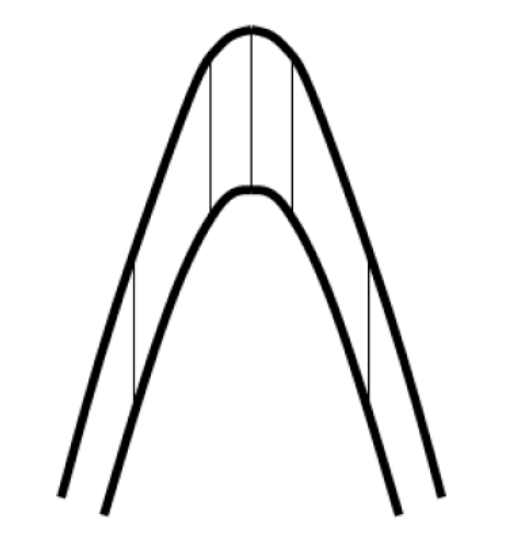
\includegraphics[width=0.3\textwidth]{pic/相似褶皱.png}
  }
  \hspace{2cm}
  \subfigure[平行褶皱]{
    \label{fig:平行褶皱}
    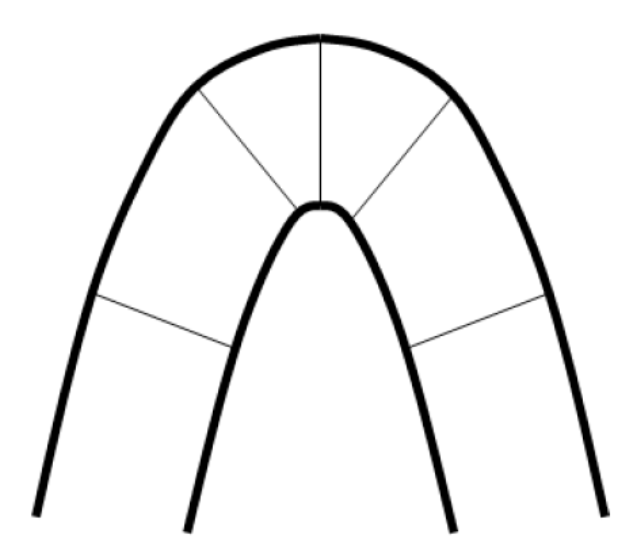
\includegraphics[width=0.3\textwidth]{pic/等厚褶皱.png}}
  
  \caption{不同几何模式的褶皱构造}
  \label{fig:不同几何模式的褶皱构造}
\end{figure}

\subsection{断层构造}

\textbf{断层构造}为岩层因构造应力发生破裂并沿破裂面发生明显位移。可分
为以下三类:
\begin{enumerate}
\item \textbf{正断层(Normal Fault):}受拉张力作用,上盘相对下降。
\item \textbf{逆断层(Reverse Fault):}受挤压力作用,上盘相对上升。
\item \textbf{走滑断层(Strike-Slip Fault):}两盘沿断层走向水平滑动。
\end{enumerate}
\begin{figure}[htbp]
  \centering
    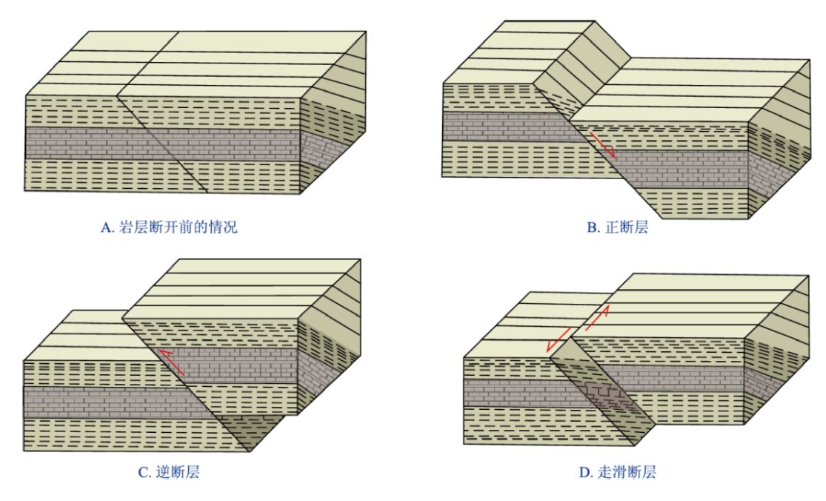
\includegraphics[width=0.6\textwidth]{pic/断层示意图.png}
  \caption{断层示意图}
  \label{fig:断层示意图}
\end{figure}

描述断层需要以下两个要素:

\begin{enumerate}
\item \textbf{断盘:}断层面两侧发生相对位移的岩体,称为断(层)盘。当
  断层面倾斜时,位于断层面上方的称为上盘,下方的称为下盘;
  当断层面近于直立时,则以方位相称,如东盘、西盘等;
  也可根据两盘相对移动的关系,把相对上升的称为上升盘,把相对下降的称为
  下降盘。

  \begin{figure}[htbp]
  \centering
    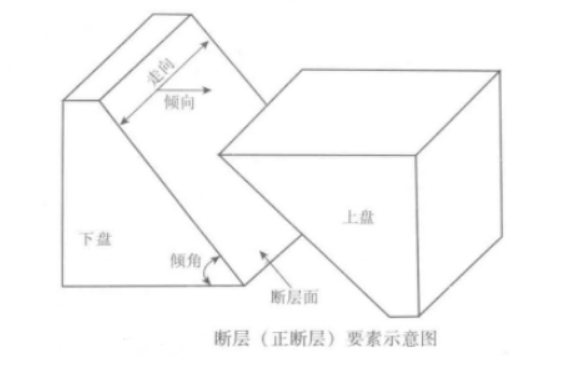
\includegraphics[width=0.5\textwidth]{pic/断层面.png}
  \caption{断层面}
  \label{fig:断层面}
\end{figure}

\item \textbf{断距:}断层两盘岩体沿断层面发生相对滑动的距离。断距的大
  小常常是衡量断层规模的重要标志,断距又分为总断距(地层断距)、水平地
  层断距及垂(铅)直地层断距。

  
\begin{figure}[htbp]
  \centering
    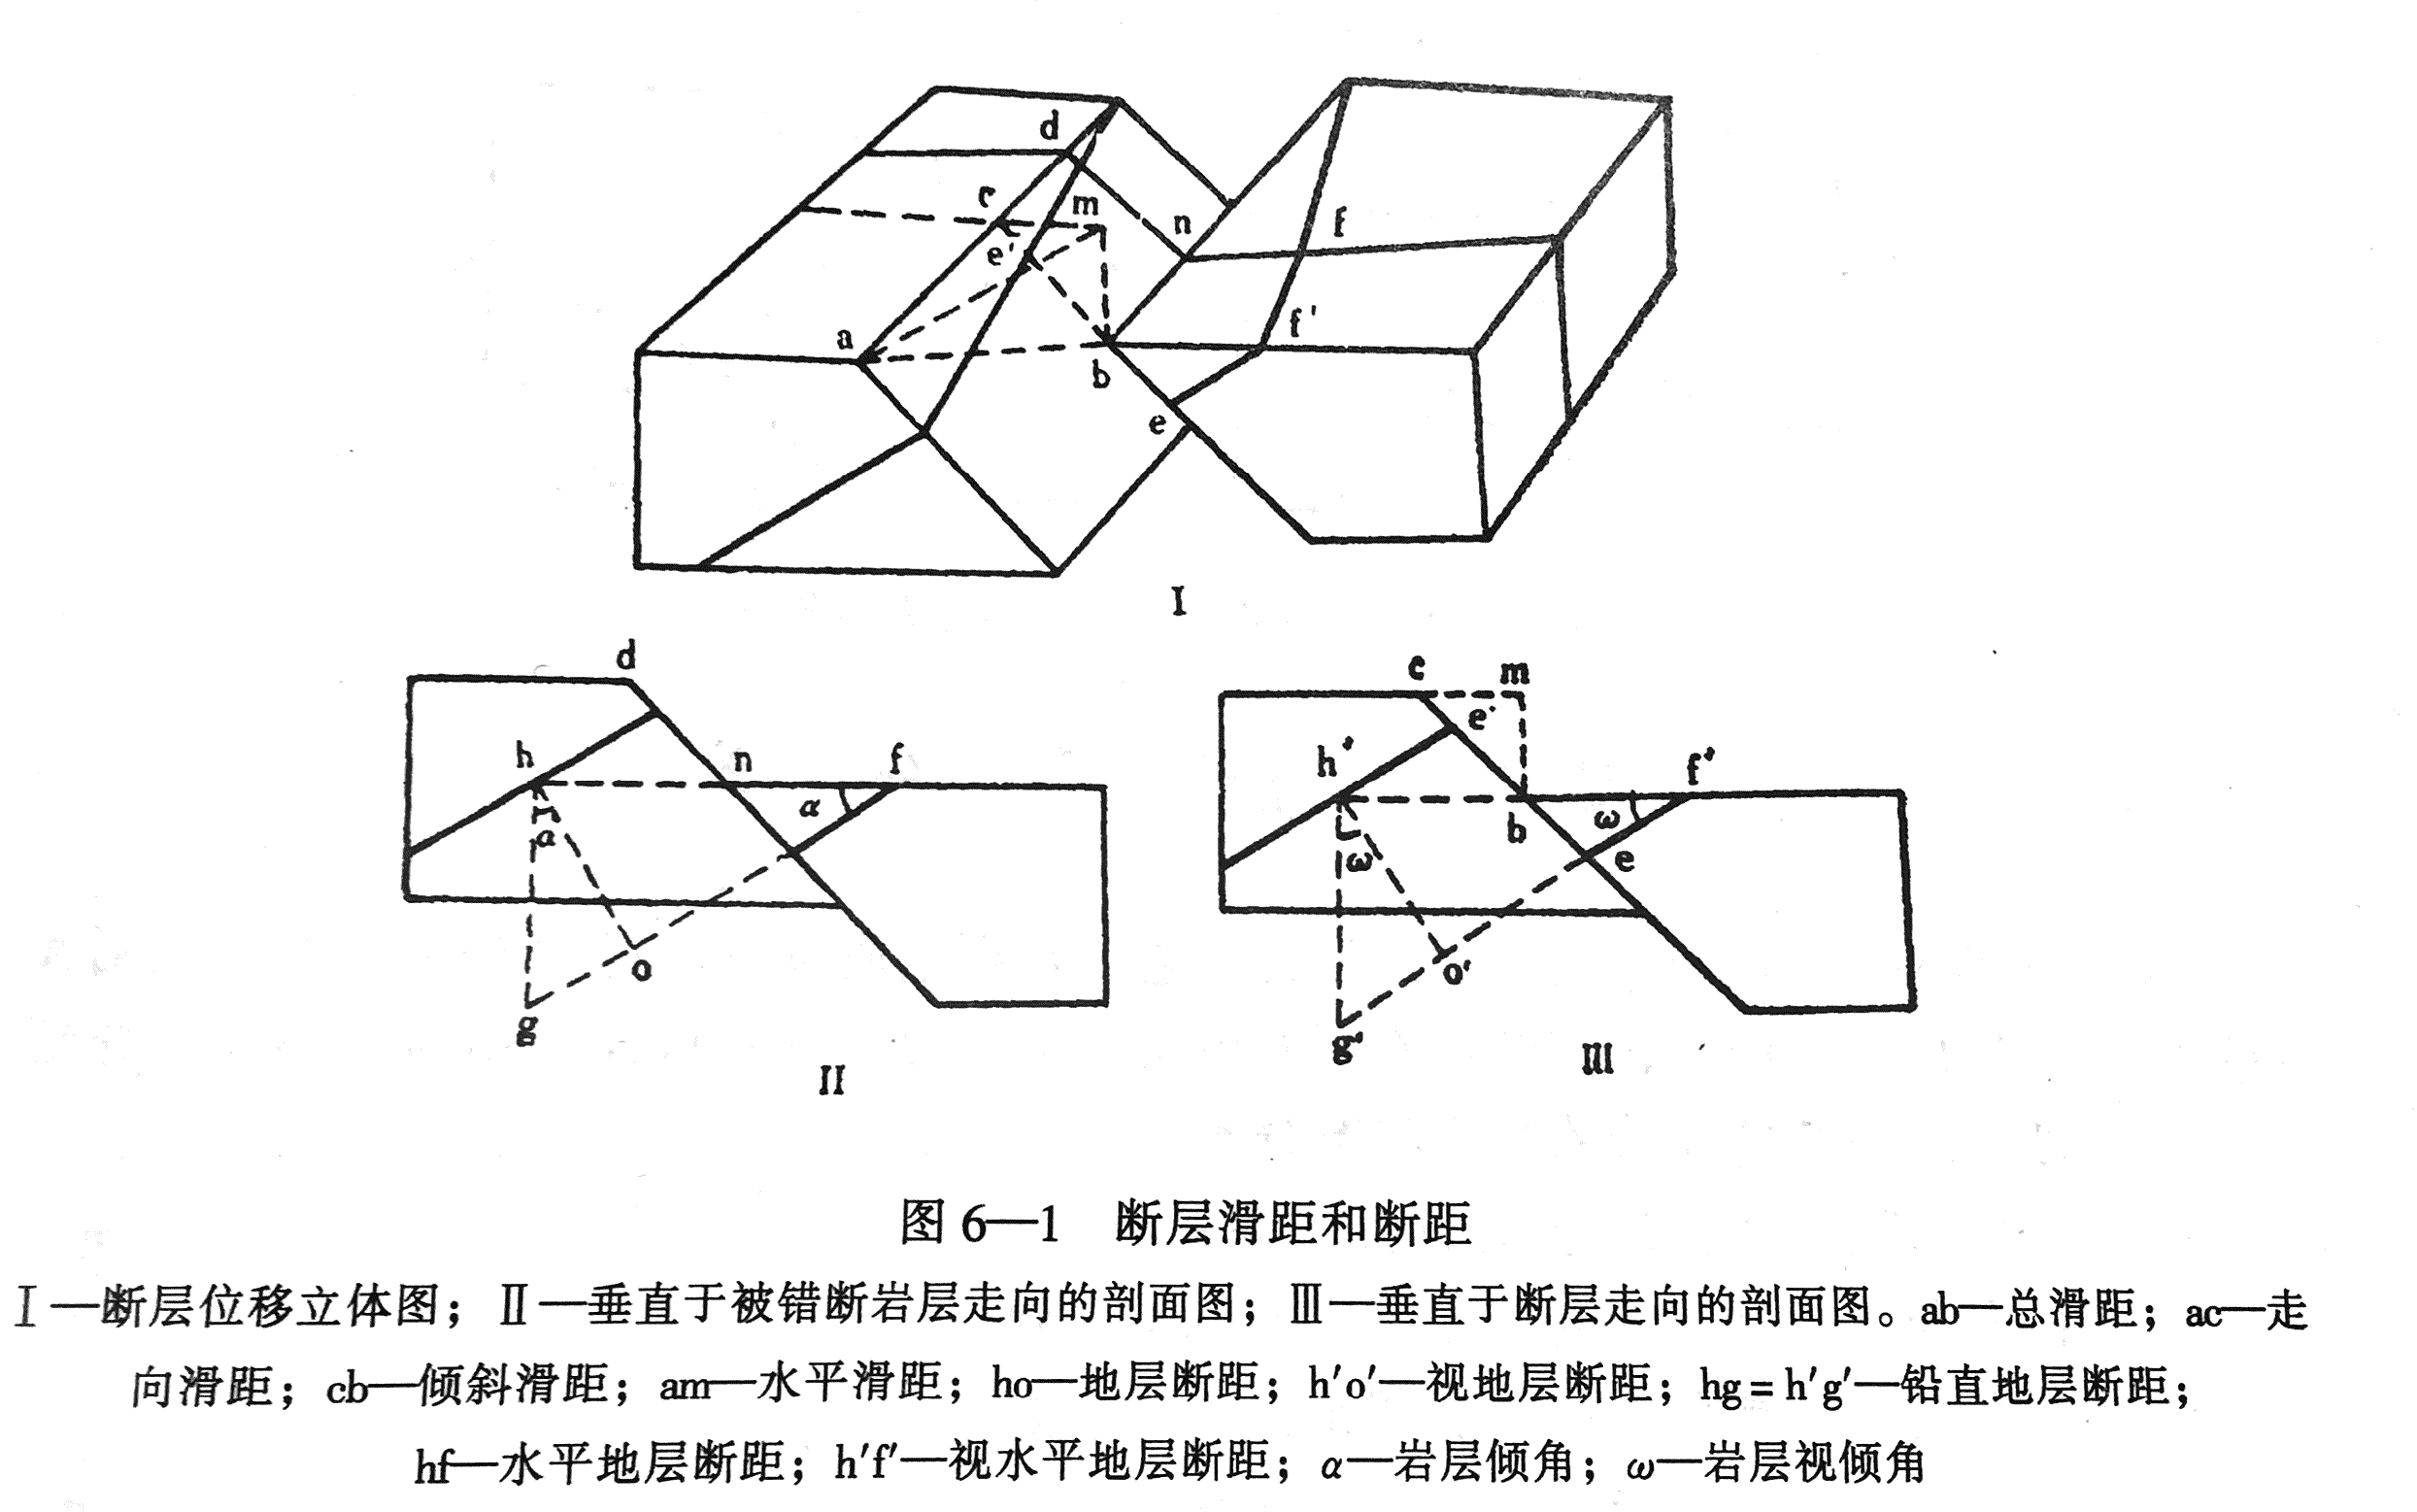
\includegraphics[width=0.9\textwidth]{pic/断层滑距和断距.png}
  \caption{断层滑距和断距}
  \label{fig:断层滑距和断距}
\end{figure}

\end{enumerate}



\subsection{岩层产状}


岩层产状是指即岩层的产出状态,由地层倾角、走向和倾向构成岩层在空间产出
的状态和方位的总称。现有的测井工具可以直接得到各个深度的岩层产状以及井
斜数据,其中:
\begin{itemize}
\item \textbf{地层倾角:}层面上的倾斜线和它在水平面上投影的夹角,也称真
  倾角,倾角的大小表示岩层的倾斜程度。
  视倾斜线和它在水平面上投影的夹角称\textbf{视倾角}。
  真倾角只有一个,而视倾角可有无数个,任何一个视倾角都小于该层面的真倾
  角。
  图\ref{fig:真倾角和视倾角}中记$ABCD$ 为地层层面,$ABEF$ 为水平面,
  $AB$、
  $CD$ 为走向线,$AFD$ 面为与走向垂直的断面,$\alpha$表示真倾角,$BD$
  作为视倾斜线则$\gamma$为视倾角。

\item \textbf{方位角:}平面上度量物体之间的角度差的方法之一,
  又称地平经度(Azimuth angle,缩写为Az)。是从某点的指北方向线起,依顺
  时针方向 到目标方向线之间的水平夹角。
方位角一般用倾向和倾角表示 ,如
  $SW205^{\circ} \angle 65^{\circ}$,即倾向为南西205度,倾角65度,其走
  向则为$NW295^{\circ}$或$SE115^{\circ}$(通常取$115^{\circ}$)。

  \begin{figure}[htbp]
  \centering
  \subfigure[方位角]{
    \label{fig:方位角}
    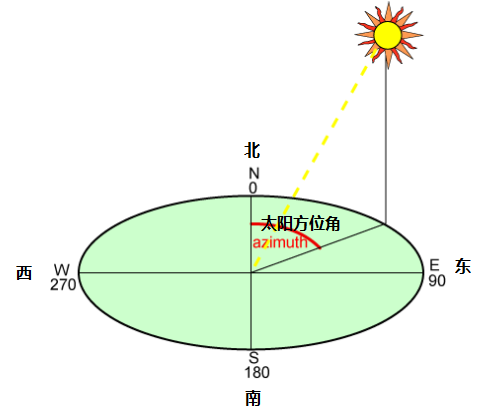
\includegraphics[width=0.4\textwidth]{pic/太阳方位角.png}
  }
  \hspace{2cm}
  \subfigure[真倾角和视倾角]{
    \label{fig:真倾角和视倾角}
    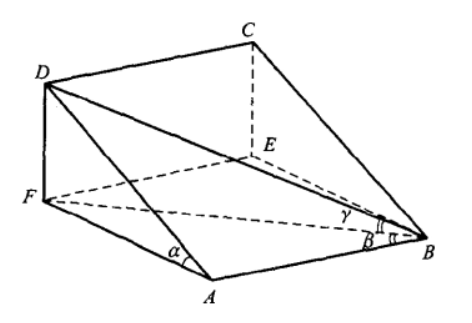
\includegraphics[width=0.4\textwidth]{pic/真倾角和视倾角.png}}
  
  \caption{方位角、真倾角和视倾角}
\end{figure}

\item \textbf{走向:}岩层层面与任一假想水平面的交线称走向线,也就是同
  一层面上等 
  高两点的连线。走向线两端延伸的方向称岩层的走向,岩层的走向也有两个方
  向,彼此相差180度,通常用小于180度的方位角表示。岩层的走向表示岩层在
  空间的水平延伸方向。

\item \textbf{倾向:}层面上与走向线垂直并沿斜面向下所引的直线叫倾斜线,
  它表示岩层的最大坡度;倾斜线在水平面上的投影所指示的方向称岩层的倾向,
  又叫真倾向,真倾向只有一个,倾向表示岩层向哪个方向倾斜。

\begin{figure}[htbp]
  \centering
  \subfigure[岩层产状]{
    \label{fig:岩层产状}
    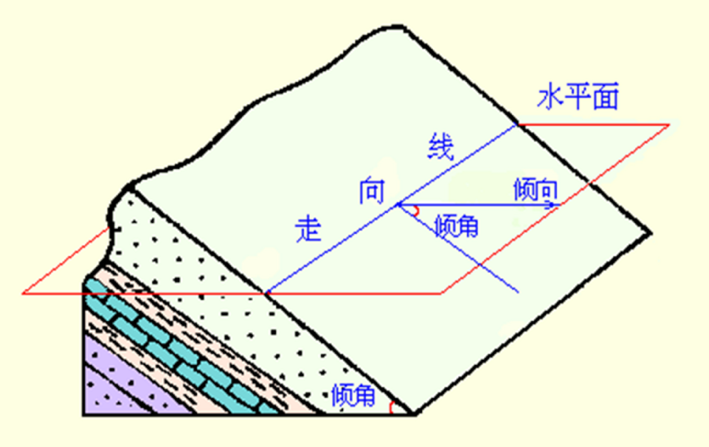
\includegraphics[width=0.4\textwidth]{pic/岩层产状.png}
  }
  \hspace{2cm}
  \subfigure[岩层产状示例]{
    \label{fig:岩层产状示例}
    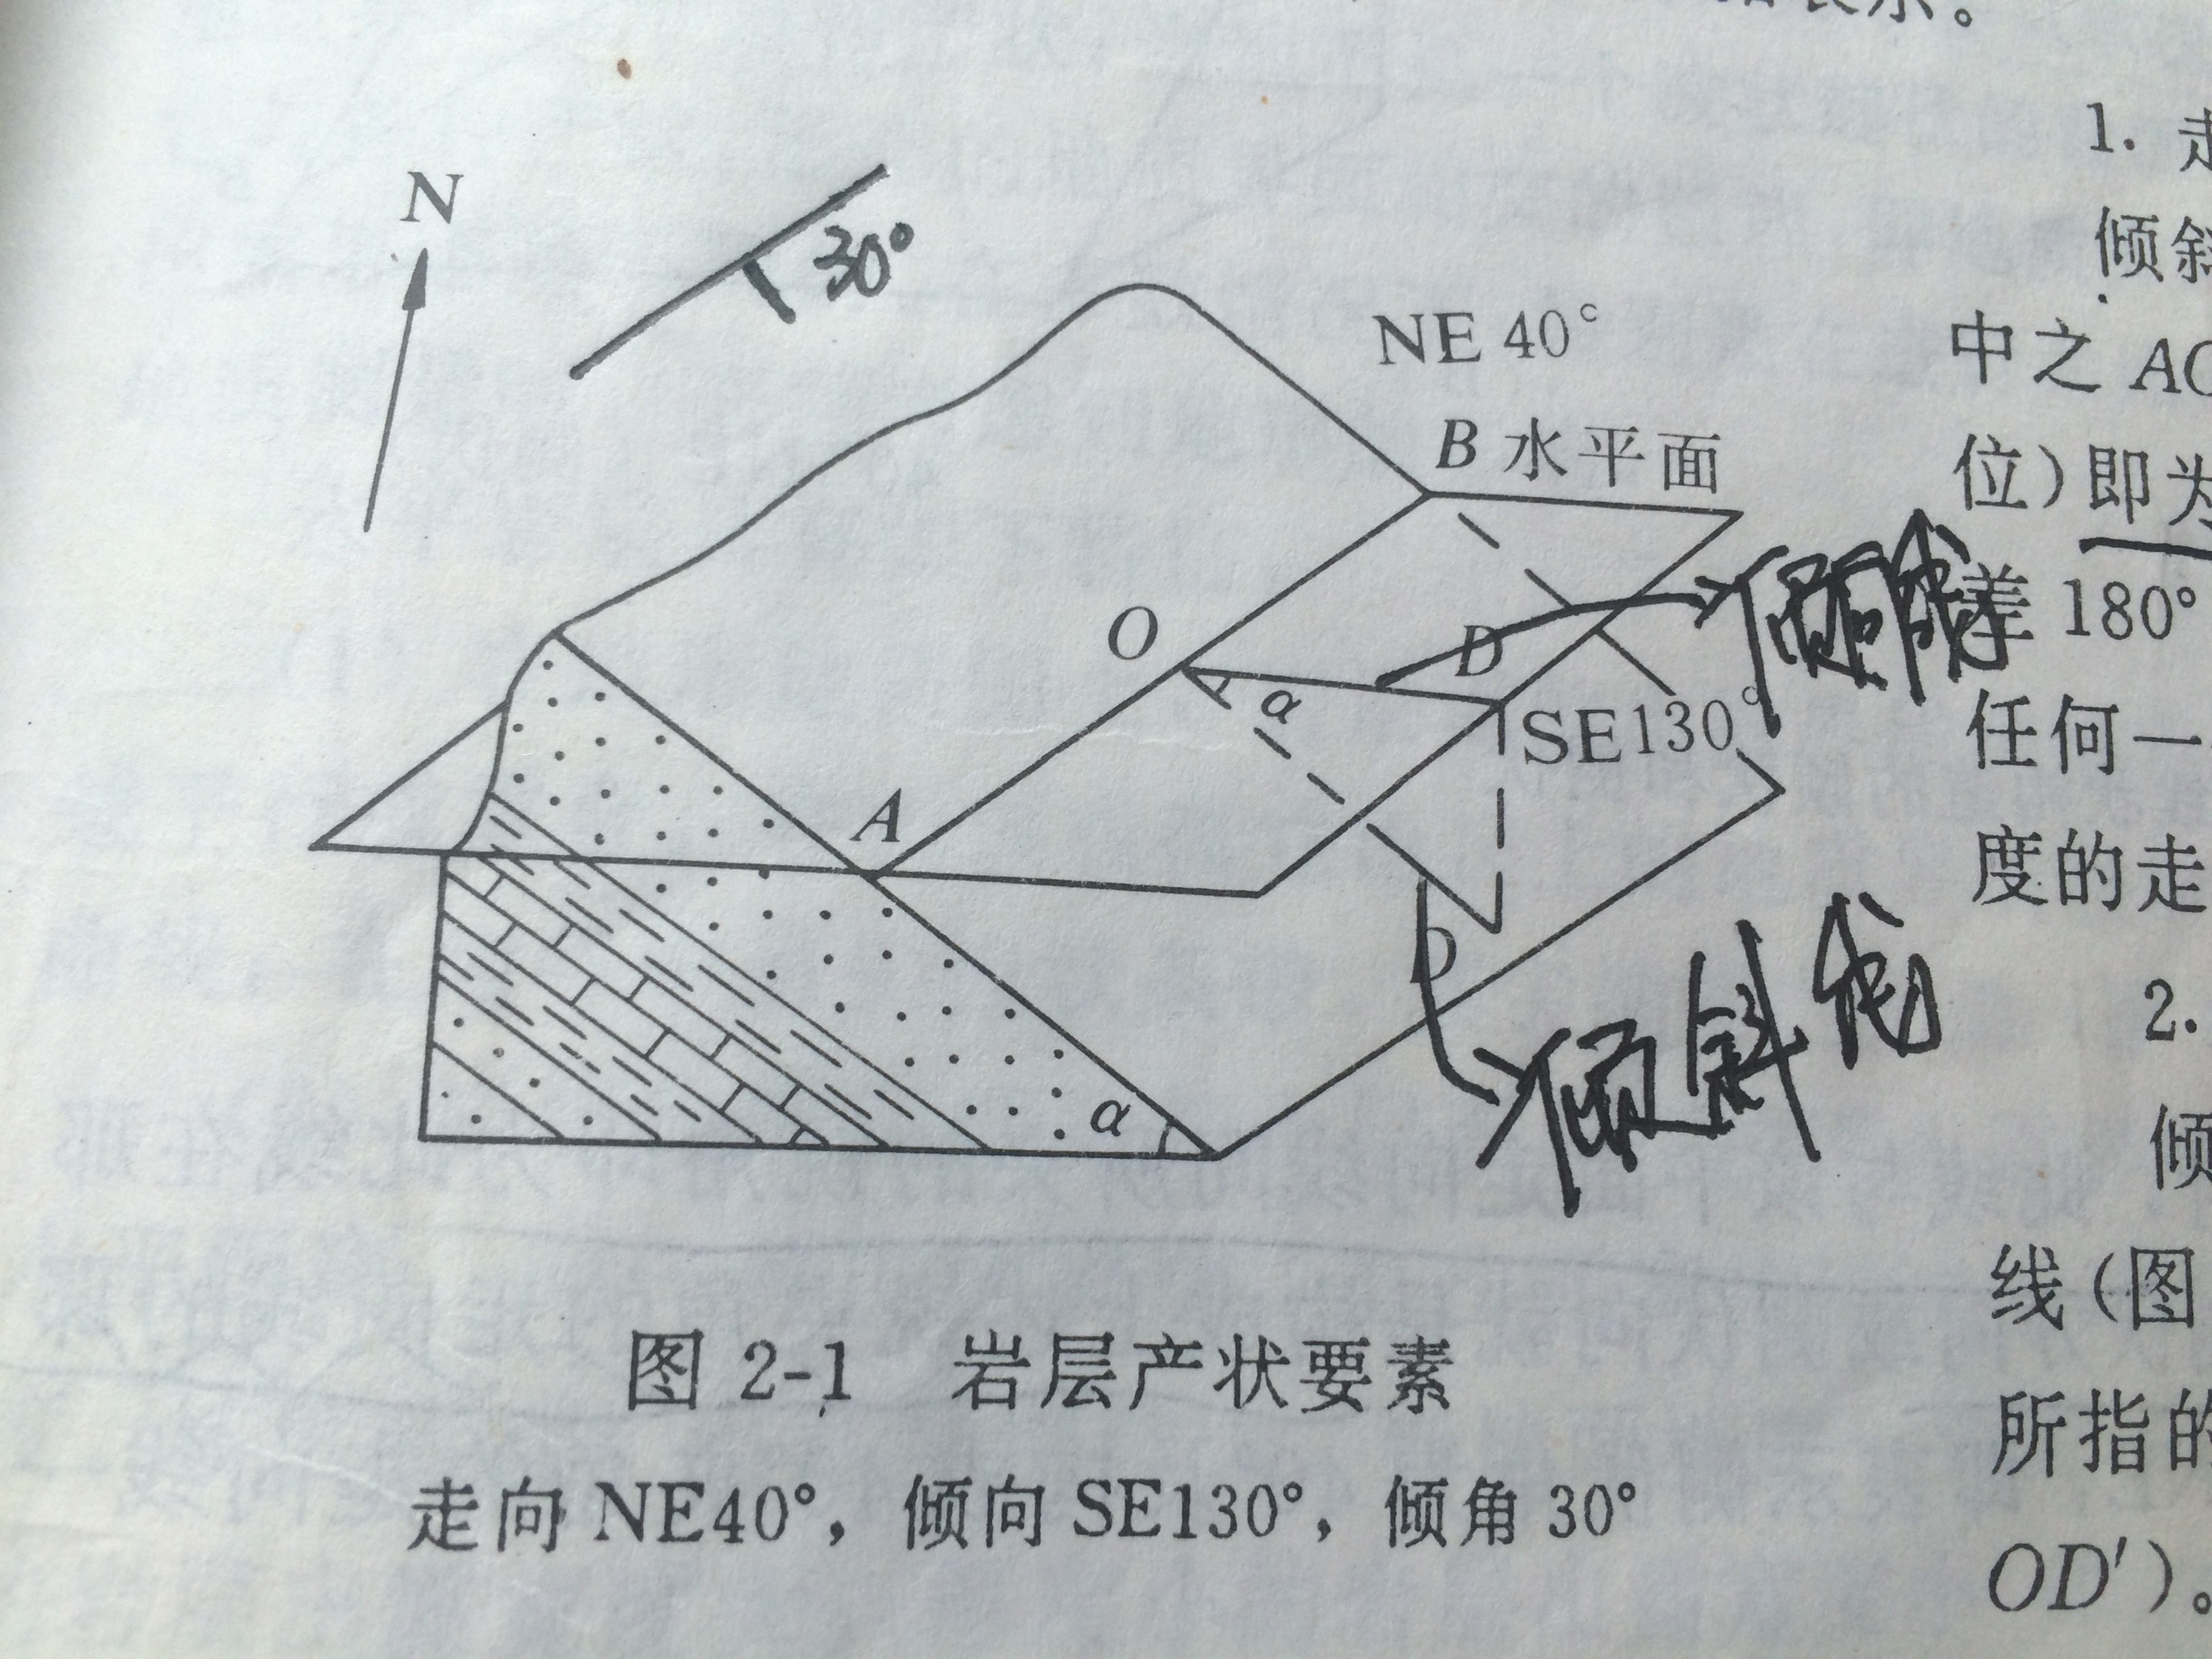
\includegraphics[width=0.4\textwidth]{pic/岩层产状示例.png}}
  
  \caption{岩层产状及其示例}
  \label{fig:岩层产状及其示例}
\end{figure}

\item \textbf{井轨迹水平投影:}将钻井轨迹投影到水平面上。
\item \textbf{井斜角:}井斜角是钻井专业术语,又叫井斜,通常定义为井眼
  轴线上某点的切线与铅垂线的夹角,井斜角通常取锐角。
\item \textbf{井斜方位角:}井眼轴线的切线在水平投影面上的方向,其中切
  线的方向取井眼前进方向。以正北方向线为始边顺时针转至该水平投影线之间
  所夹的角度来表示井斜方位角。

  \begin{figure}[htbp]
  \centering
  \subfigure[井轨迹投影]{
    \label{fig:井轨迹投影}
    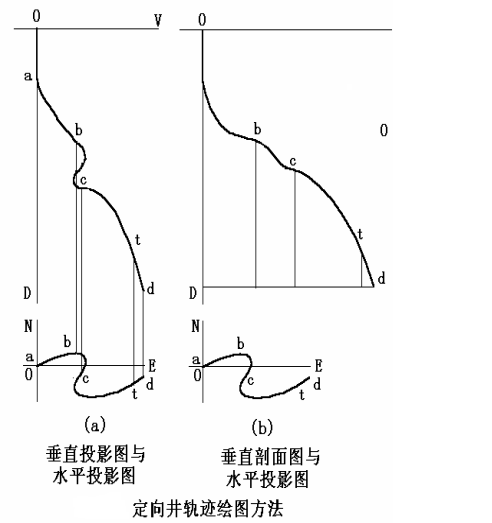
\includegraphics[width=0.4\textwidth]{pic/井轨迹投影.png}
  }
  \hspace{1cm}
  \subfigure[井斜角和井斜方位角]{
    \label{fig:井斜角和井斜方位角}
    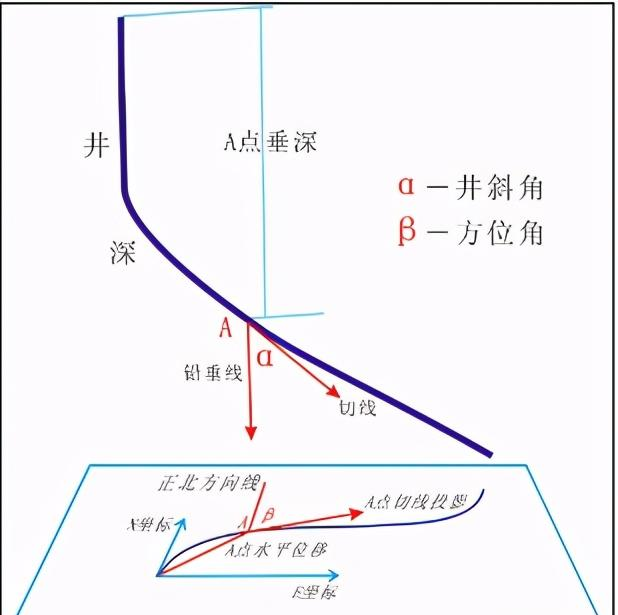
\includegraphics[width=0.4\textwidth]{pic/井斜角和井斜方位角.png}}
  
  \caption{井斜相关概念}
  \label{fig:井斜相关概念}
\end{figure}
\end{itemize}

\subsection{施密特网}
\label{sec:施密特网}

\subsubsection{赤道方位等积投影}

\textbf{施密特网图(Schmidt Net)}是基于赤道方位等积投影构建的等面积网
格系统,用于地质学中的方向数据分析(如岩层节理、断层倾向),该等积投影
方法核心步骤如下:
\begin{enumerate}[步骤1:]
\item  定义单位球面方程
  \begin{displaymath}
    x^2+y^2+(z-1)^2=1,
  \end{displaymath}
球心位于$(0,0,1)$,投影平面为 $z=0$,切点为原点 $O(0,0,0)$,后续仅取球体下
半部分($z\leq 1$)用于构造施密特网,也可以取上半球体,步骤相同。 
\item 对球面上任意点 $P$,过 $P$、原点 $O$ 和球极 $(0,0,2)$ 作大圆平面。
\item 以 $O$ 为圆心,$OP$为半径,在包含 $OP$ 的大圆平面上作圆弧,与投影平面相交得
  投影点$P'$。
\end{enumerate}

图\ref{fig:兰伯特等积投影}为等积投影方法示例,球面上曲线$ABCDE$通过等
积投
影形成曲线$A'B'C'D'E'$。等积性的核心在于球面上任意区域的面积与其在投影
平面上对应区域的面积相等。
在该示例中,平面$AOE$逆时针转动到倾斜面$ACE$的过程中扫过的
球面面积等于投影平面上$A'B'C'D'E'$围成的面积。

\begin{figure}[htbp]
  \centering
    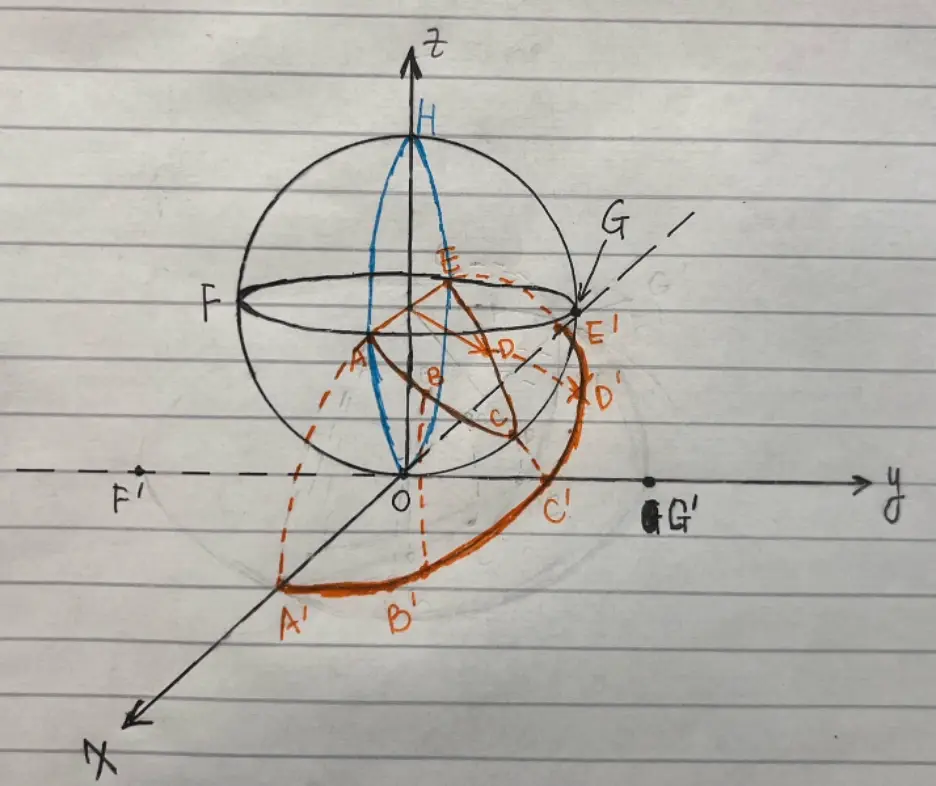
\includegraphics[width=0.45\textwidth]{pic/兰伯特等积投影.png}
  \caption{兰伯特等积投影示例}
  \label{fig:兰伯特等积投影}
\end{figure}

\subsubsection{施密特网}

施密特网通过构建标准化等面积网格,将抽象投影原理转化为可测量的工具。
如下图所示,其中所有连接南北两极的曲线段和直线段都是网图的大圆,下图红
色曲线段表示,可以理解成施密特网图的“经线”;连接南北两极的直线段称为
中央经线。此外,连接东西两极的直线段,即施密特网图的“赤道”,也是大圆。
所有除赤道的东西走向曲线段称作施密特网图的小圆,下图蓝色曲线段表示,可
以理解成网图的“纬线”。

\begin{figure}[htbp]
  \centering
    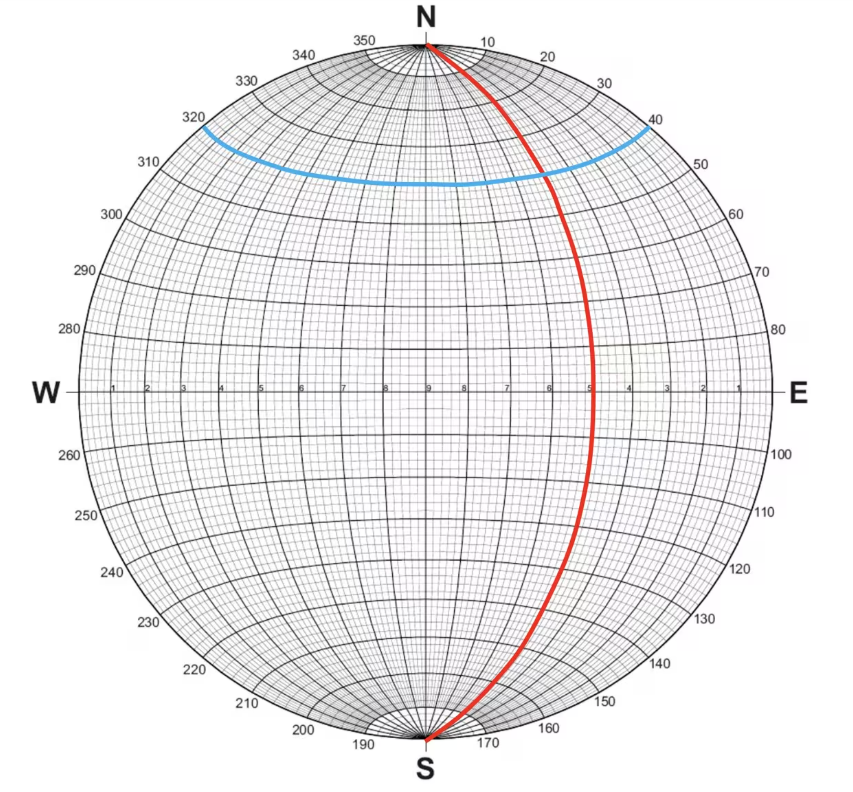
\includegraphics[width=0.45\textwidth]{pic/施密特网.png}
  \caption{施密特网}
  \label{fig:施密特网}
\end{figure}

在地质构造分析中,常将地质面的法线方向(也称为极点)投影到施密
特网中,通过极点位置分布来进行识别:若极点高度集中,则表示倾向与倾角分
布稳定,即为单斜构造;若极点沿单一经向大圆弧连续分布,则为圆柱状褶皱,
否则为非圆柱状褶皱。

\subsection{极射赤平投影与吴氏网}

\subsubsection{极射赤平投影}
极射赤平投影是一种以球面投影为基础的几何方法,通过将三维空间中的方向、
平面或线投影到一个参考平面(通常为赤道平面),形成二维图形,保留原始结
构的空间关系。 投影方式类似于复变函数的黎曼面构造,唯一的区别是极射赤
平投影中下半球投影使用上极射点发出射线,上半球投影使用下极射点发出射线。
例如图\ref{fig:极射赤平投影图}中线$PB$投影到赤平面上为$OB'$,
将倾斜面$NBS$与球面的无数个交点与$P$点连成直线
并投影到赤平面得到弧线$NB'S$。   

\begin{figure}[htbp]
  \centering
    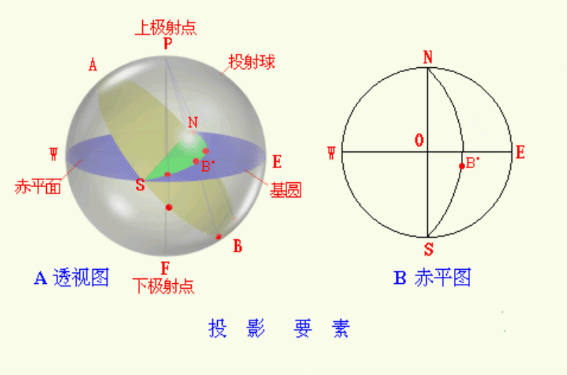
\includegraphics[width=0.55\textwidth]{pic/级射赤平投影图.png}
  \caption{极射赤平投影图}
  \label{fig:极射赤平投影图}
\end{figure}

\subsubsection{吴氏网}

吴氏网(立体网)是一种基于等角极射赤平投影的网格工具,用于将三维空间中
的方向、平面和线投影到二维平面上,同时保持原始角度关系不变,见图
\ref{fig:极射赤平投影得到吴氏网},可以理解为带刻度的赤平图。

图\ref{fig:极射赤平投影得到吴氏网}(A)中吴氏网的经线可以用
图\ref{fig:极射赤平投影得到吴氏网}(B)的下半圆球面与过圆心的倾斜大圆
(倾斜面)的交线(也就是相交得到的空间曲线)按极射赤平投影法投影在赤平
面(图B中的半球切面)形成的弧线得到。 
同理,吴氏网的纬线可由下半圆球面与不过圆心的直立小圆的交线形成的空间曲
线投影在赤平面投出的弧线得到。

吴氏图中从N向顺时针360度标方位,代表倾斜平面的倾向。
经线弧$NES$到弧$NS$之间的一系列弧线分别对应倾斜平面倾角0度到90度,
经线弧$NWS$到弧$NS$之间的一系列弧线也分别对应倾斜平面倾角0度到90度。

\begin{figure}[htbp]
  \centering
    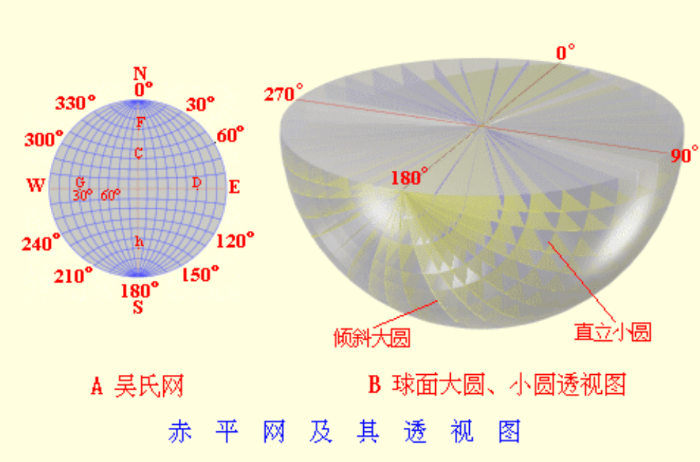
\includegraphics[width=0.6\textwidth]{pic/极射赤平投影得到吴氏网.png}
  \caption{极射赤平投影得到吴氏网}
  \label{fig:极射赤平投影得到吴氏网}
\end{figure}

\subsubsection{利用吴氏网读取倾斜面的倾角倾向信息}

当倾斜面极射赤平投影到吴氏网后,圆弧与$WE$线相交的点对应的刻度即为该倾
斜面的倾角。连接圆弧两端点并向圆弧方向做垂直平分线,
该垂直平分线与吴氏图边界相交的点对应的刻度即为该倾斜面的倾向。

例如,
图\ref{fig:利用吴氏网进行极射赤平投影}为倾斜面$NDS$与倾斜面法线(法向
量)$OF$的极射赤平投影示例:
法线$OF$投影到赤平面上得到该倾斜面$NSD$的极点$F'$, 
$D'E$表 示倾斜面倾角大小$40^{\circ}$(B图弧$ND'S$对应吴氏网
$40^{\circ}$经线),同理$WF'$表示法线倾角大小为$50^{\circ}$($WE$处的
纬线(也是赤道线)与$50^{\circ}$经线交点)。 

\begin{figure}[htbp]
  \centering
    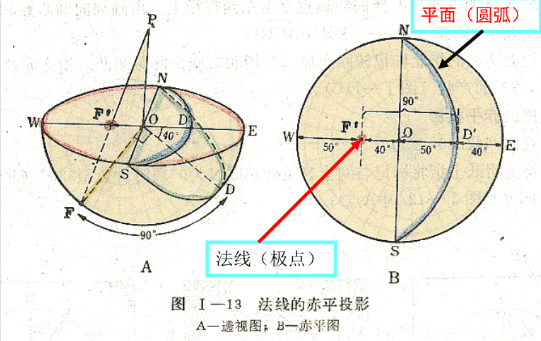
\includegraphics[width=0.6\textwidth]{pic/平面法向量直线投影.png}
  \caption{利用吴氏网进行极射赤平投影}
  \label{fig:利用吴氏网进行极射赤平投影}
\end{figure}

\subsection{构造轴线与构造剖面}

\subsubsection{构造轴线}

褶皱的构造轴线又叫\textbf{褶皱轴(Fold Axis)},也是褶皱中岩层弯曲的
\textbf{枢纽线}(枢纽的延伸方向)。
\textbf{轴面(Axial Plane)}为平分褶皱两翼的假想平面,枢纽线通常位于轴
面内,如图\ref{fig:褶皱构造图示}所示:

\begin{figure}[htbp]
  \centering
    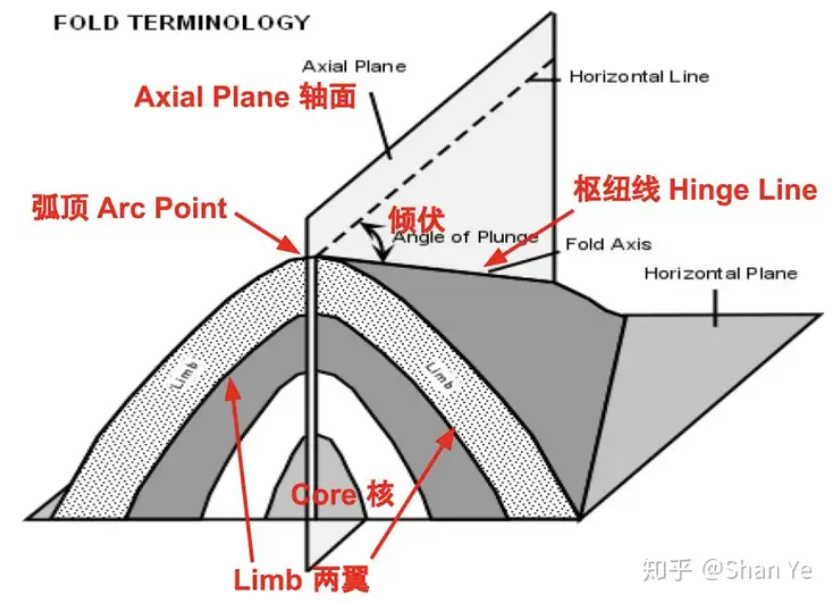
\includegraphics[width=0.6\textwidth]{pic/褶皱构造图示.png}
  \caption{褶皱构造图示}
  \label{fig:褶皱构造图示}
\end{figure}

\subsubsection{构造轴线与投影平面计算}
\label{sec:构造轴线与投影平面计算}
单斜构造的构造轴线通常是走向线,断层的构造轴线是断层带的主破裂
面走向线或多条断层的平均走向线,投影平面与构造轴线垂直。

枢纽线水平的褶皱构造可使用$\pi$图法确定构造轴线:
\begin{enumerate}
\item 从数据中得到褶皱上多处切平面的产状,并根据产状通过极射赤平投影得
  到各切平面法向量($P_i$)在赤平面(吴氏网)上的投影点。 
\item 使用最小二乘法将多个法向量的投影点在赤平面上拟合一个大圆,该大圆
  对应的平面即是投影面($\pi$圆面),构造轴线,也是该投影面的法线
  $\beta$倾向与投影面相反,倾角为投影面倾角的余角。
\end{enumerate}

后续将该投影面或与其平行的平面作为二维地质构造剖面。
 \begin{figure}[htbp]
  \centering
    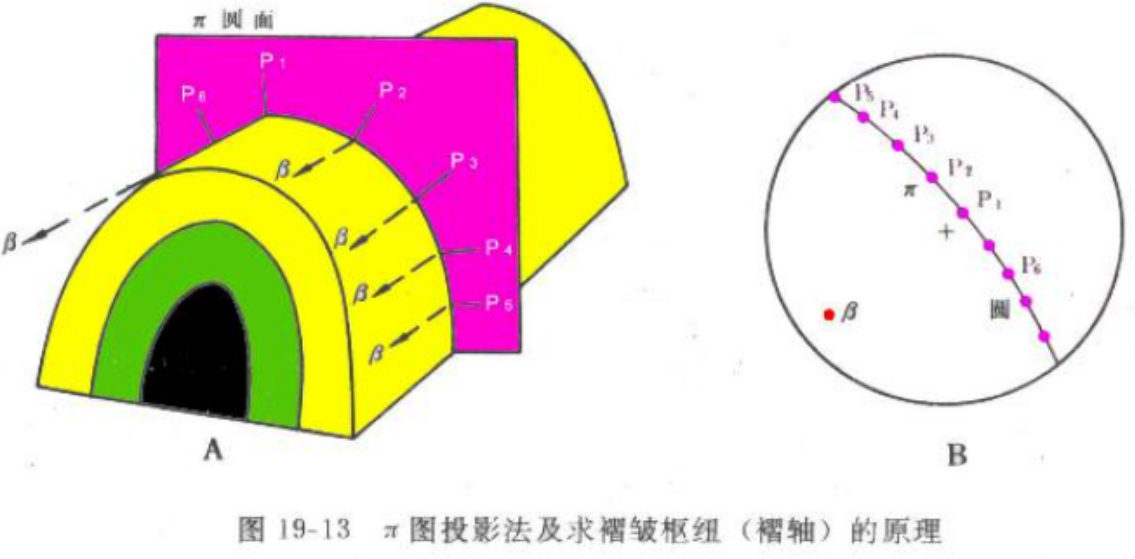
\includegraphics[width=0.8\textwidth]{pic/图解法求褶皱枢纽.png}
  \caption{$\pi$图法计算褶皱枢纽示例}
  \label{fig:图解法求褶皱枢纽}
\end{figure}

\subsection{蛛网法}
\label{sec:蛛网法}
蛛网法可以根据给定岩层产状和构造轴线来生成二维构造剖面,其主要步骤为:
\begin{enumerate}
\item 根据井筒轨迹上的倾角数据生成导向网,初始导向网由相邻两倾角的垂线
  之间的角平分线构成,这些平分线位于两倾角的中点处,
  见图\ref{fig:蛛网法}(b)。
  为了在下一步中最大限度地利用输入数据延伸地层,还在初始网集中额外加入
  了最顶端和最底端倾角的垂线。初始经向丝的数量等于初始倾角数加一。
  导向网的构建则通过以下迭代合并这些初始经向丝来完成:
  \begin{enumerate}[步骤1:]
  \item 在当前的经向丝集合$T_{1}, T_{2}, T_{3}, \ldots, T_{N}$中,计算
    每对相邻丝$T_{n}$与$T_{n+1}$的所有交点$I_{1}, I_{2}, I_{3},
    \ldots, I_{N+1} $,见图\ref{fig:蛛网法}(c)。 
  \item 在这些交点中,找到距离井筒最近的交点$I_{n}$,
    见图\ref{fig:蛛网法}(c)中圈出的交点。
  \item 在该交点处停止经向丝$T_{n}$和$T_{n+1}$的延伸,并从此交点开始生
    成一条新的经向丝$T_{\text {new }}$,新生成的经向丝方向定义为位于
    $T_n$上方倾角和$T_{n+1}$下方倾角的垂线的平分线(这里n从上到下排序)。
    见图\ref{fig:蛛网法}(d)。 
  \item 更新经向丝集合:移除$T_{n}$和$T_{n+1}$,并将新生成的$T_{\text
      {new }}$加入集合。 
  \item 当不再出现新的交点,或集合内仅剩一条经向丝时,迭代结束,见图
    \ref{fig:蛛网法}(g)。
  \end{enumerate}
  \item  
    这些经向丝将二维平面划分为若干区域,每个区域包含一个倾角,
    再针对每个数据探测点生成一条分段直线轨迹,
    该轨迹在二维平面内的延伸遵循:直线以当前区域倾角持续延伸,直至触及
    当前区域边界;当直线延伸至区域边界时,自动切换为相邻新区域的倾角,
    并以此倾角继续延伸,见图\ref{fig:蛛网法}(h)。
  \end{enumerate}
  该方法对于垂直井中包含平行褶皱的平行层构建以及水平井中的单斜构造都非
  常有效。

 \begin{figure}[htbp]
  \centering
    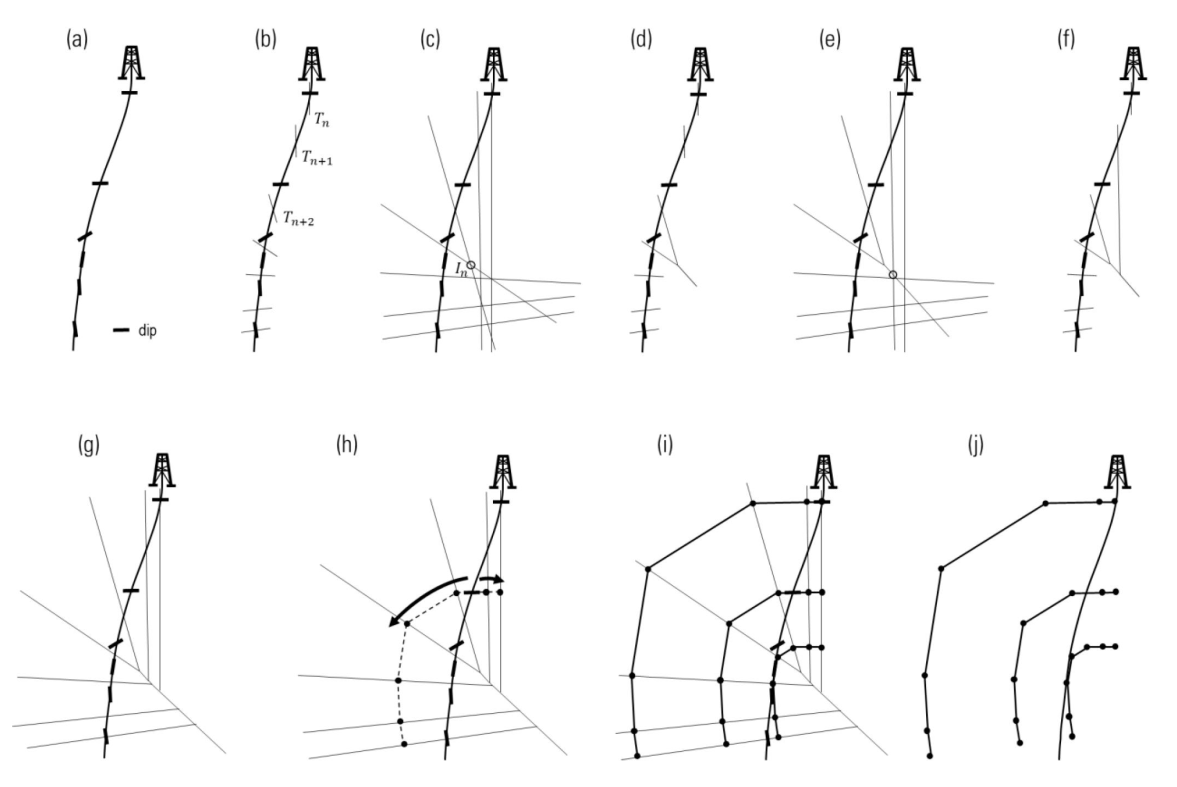
\includegraphics[width=\textwidth]{pic/蛛网法.png}
  \caption{蛛网法示例}
  \label{fig:蛛网法}
\end{figure}


\section{项目契约}

目前第一步的目标是针对单斜构造构建二维地质剖面,长远目标为针对任意构造
构建二三维地质剖面。

\begin{itemize}
\item \textbf{初步目标的输入数据:}一份垂直井的测井数据,其中包括以下
  几列:
  DEPT(垂深),DEVI(井斜角),DPAZ(地层倾角倾向),
  DPTR(地层倾角角度),HAZI(水平方位角),
  TYPE(地层构造类型)。另外用户也可以自定义的构造轴线,若缺省则默认
  根据按照章节\ref{sec:构造轴线与投影平面计算}计算构造轴线。
\item \textbf{初步目标的输出数据:} 二维单斜地质剖面图。
\end{itemize}

\section{技术路线}

算法总体框架主要分为数据过滤和构造剖面生成两部分。算法均为初步设计,后
续可根据实际情况不断进行改进。

\subsection{数据过滤}

针对给定的测井数据,要进行以下处理:
\begin{enumerate}[步骤 1:]
\item 数据预处理:根据地质年代信息确定地质分层边界,在同一套地层中,选
  择适当的数据条数进行分组处理,针对每个分组求平均倾角和平均倾向,并赋
  值给每条数据。另外,若用户有指定的断层部分,则直接对这部分数据进行标
  记,不再进行后续的分类。
\item 突变点识别:将地层倾角或倾向突然发生剧烈变化(默认超过10度,用
  户可自定义)的深度点记为突变点,并将突变点信息加入候选列表。
\item 断层破碎带识别:如果候选列表中有连续5个(默认,用户可自定义)
  以上的深度点均为突变点,则将该区域记为断层破碎带区域。用户可以选择对
  该层区域进行剖面构造或者直接剔除该部分数据,默认为进行剖面构造。
\item 断层构造识别:判断牵引构造,在候选列表中选择除判断为破碎带之外的
  各条数据,如果该数据的上下盘(默认前5个和后5个数据)的平均倾向呈钝角
  (大于90度)或者上下盘倾角差距大于默认的阈值,则判定为断层。其余候选
  列表中的点判断为噪声。
\item 数据分层:将噪声过滤掉后,数据可以分为若干个断层破碎带、断层构造
  以及稳定区域。 
\end{enumerate}

测井数据中可能会存在多个稳定区域,因为某地质区域的各个地层走向大致不一
致(如沉积了多套不同走向的地层),则需要根据走向的不同区分不同套的地层,
后续在每一套走向大致相同的地层上分别生成二维构造剖面。

\subsection{构造剖面生成}

构造剖面生成步骤如下:
\begin{enumerate}[步骤 1:]
\item 分区和模型选择:如果测井数据中提供地层构造模型(TYPE)则不需要该步
  骤,否则需利用施密特网对各稳定区域进行构成分析,依照极点分布特征选取
  不同的地层构造模型。 
\item 按照章节\ref{sec:构造轴线与投影平面计算}计算各区域的构造轴线和构
  造剖面所在平面,若后续测井数据提供构造轴线数据,则不需要该步骤。
\item 利用章节\ref{sec:蛛网法}中的蛛网法生成构造剖面。
\item 若用户指定在某过井平面生成剖面,则将构造剖面向该平面进行投影即可。
\end{enumerate}

\subsection{简化情况:二维单斜构造剖面生成}

由于初步目标仅为针对二维单层单斜地层生成构造剖面,因此算法可以进行相应
的简化:
\begin{enumerate}[步骤 1:]
\item 过滤掉地层倾角或倾向突然发生剧烈变化(默认为超过10度)的测井数据,
  并对测井数据进行粗化,保证相邻深度点的深度差不低于1米。
\item 使用蛛网法生成二维地质剖面。
\end{enumerate}

\section{项目整体规划}
项目主要分为五个阶段:
\begin{enumerate}[第1阶段:]
\item 针对单斜构造生成二维构造剖面;
\item 针对任意自定义构造剖面线(垂直于构造轴线并与其保持至少10度的夹角)
  生成单斜二维构造剖面;
\item 针对褶皱和断层等复合地质生成二维构造剖面;
\item 支持生成倒转褶皱形态的二维构造剖面;
\item 为大斜度井和水平井生成二维构造剖面,在此基础上进行储层预测。
\end{enumerate}

\section{问题方案}
\subsection*{1. 地层投影线的尖灭}
\begin{itemize}
  \item \textbf{尖灭的概念}\\
  指一个地层(或岩层、矿层、沉积体等)在其延伸方向上,厚度逐渐变薄,最终完全消失的现象。通俗来说这就像一根楔子插入地下,一端厚,另一端逐渐变薄到零。
  
  \item \textbf{"尖灭问题"的核心难点:}\\
  确定尖灭点的位置,这是最核心的问题。地层从有到无,这个"消失点"(尖灭点)的位置,在缺乏足够密集的观测点(露头、钻孔)的情况下,精确判断尖灭点的位置非常困难,往往存在很大的推测性和不确定性。
  
  \item \textbf{投影线的形态}
  \begin{itemize}
    \item \textit{自然收敛:} 对于沉积尖灭,投影线应该自然、平缓地收敛闭合,形成一个尖灭点(或尖灭线)。绘制的难点在于如何平滑合理地连接有限的观测点,真实反映地层厚度渐变消失的趋势。
   
    \begin{figure}[htbp]
      \centering
      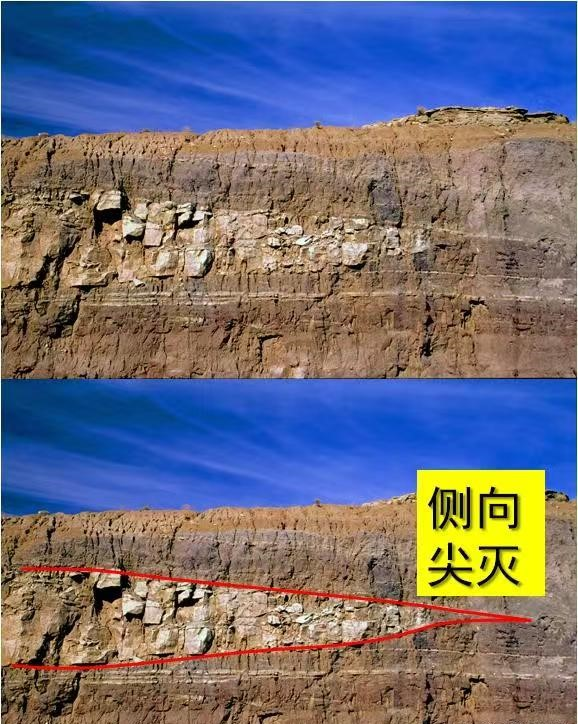
\includegraphics[width=0.6\textwidth]{pic/投影线尖灭.jpg}
      \caption{投影线尖灭}
      \label{fig:投影线尖灭}
    \end{figure}
    
    \item \textit{截断:} 对于剥蚀尖灭,投影线是被一个剥蚀面(也称不整合面体)截断的。绘制的难点在于准确确定不整合面的位置和形态,以及地层线如何被其截断。例如下图接近水平的青色地层和多个倾斜的粉色、绿色、深蓝色地层呈现角度关系,这些粉色、绿色、深蓝色地层被截断。
    
    \begin{figure}[htbp]
      \centering
      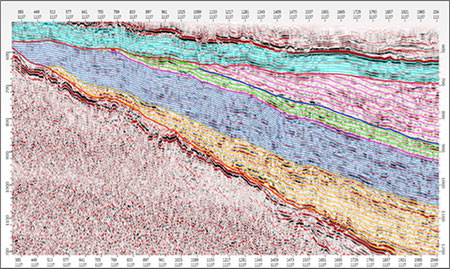
\includegraphics[width=0.6\textwidth]{pic/剥蚀尖灭.png}
      \caption{剥蚀尖灭}
      \label{fig:剥蚀尖灭}
    \end{figure}
  \end{itemize}
  
  \item \textbf{解决方法}
  \begin{enumerate}
    \item 如尖灭示意图所示,如果拟合的地层界面线相交则出现尖灭,交点为尖灭点(直观方法)
    \item 根据地层法向量的变化来判断(假想方法)
  \end{enumerate}
\end{itemize}

\subsection*{2. 投影线合并问题及投影后地层界面平滑问题}
\begin{itemize}
  \item \textbf{法线投影解释}\\
  核心是一种将三维空间的地层产状"翻译"到二维剖面图上的方法,法线就是地层切平面法向量所在的直线。
  
  \begin{itemize}
    \item \textit{法线投影是用来解决以下问题:}\\
    三维现实是地下有一个倾斜的地层层面(比如一个背斜的翼部)。这个层面在三维空间中有一个确定的倾向(朝哪个方向倾斜)和倾角(倾斜的角度)。所需的二维剖面是地质学家需要在图纸或电脑屏幕上绘制一个垂直剖面图(通常是沿着某个特定方向切割地下的切面图),这个图是二维的。目标是如何把三维空间中测量到的、位于井筒中某个点的地层真倾角/倾向,准确地表示在这个二维的垂直剖面图上?直接画真倾角通常是错误的,因为剖面方向不一定与地层倾向方向平行。
    
    \item \textit{法线投影的原理:}\\
    法线与垂直方向(铅垂线)之间的夹角,就等于该地层的真倾角。\\
    投影的目标不是直接把倾斜的地层线画在剖面上,而是把代表该地层方向的法线,"正交投影"到我们关心的那个垂直剖面平面上。
    
    \item \textit{投影过程:}
    \begin{enumerate}
      \item 确定法线向量。根据井中测得的该深度点的地层真倾角 ($\alpha$) 和真倾向 ($\beta$),可以计算出该点地层法线在三维空间中的方向向量。
      \item 确定剖面方向。明确你要绘制的是哪个方向的垂直剖面(例如,剖面方位角是 $120^\circ$)。
      \item 投影法线到剖面平面。将三维的法线向量,正交投影(通俗解释就像正午阳光垂直照射物体投下影子到纸面上)到指定的垂直剖面平面上。
      \item 获取视倾角。投影后落在剖面平面上的这条线,就是法线在剖面平面上的投影线。这条投影线与剖面平面内的垂直方向线(铅垂线)之间的夹角,称为该地层在这个特定剖面方向上的视倾角 ($\alpha'$)。
      \item 在剖面图上表示。在垂直剖面图上,在对应的深度点处,画一条与铅垂线成 $\alpha'$ 角的直线(其方向由投影线的方向决定)。这条线就代表了该点地层在所选剖面方向上看起来的倾斜方向和角度(视倾角/视倾向)。
    \end{enumerate}
    
    \begin{figure}[htbp]
      \centering
      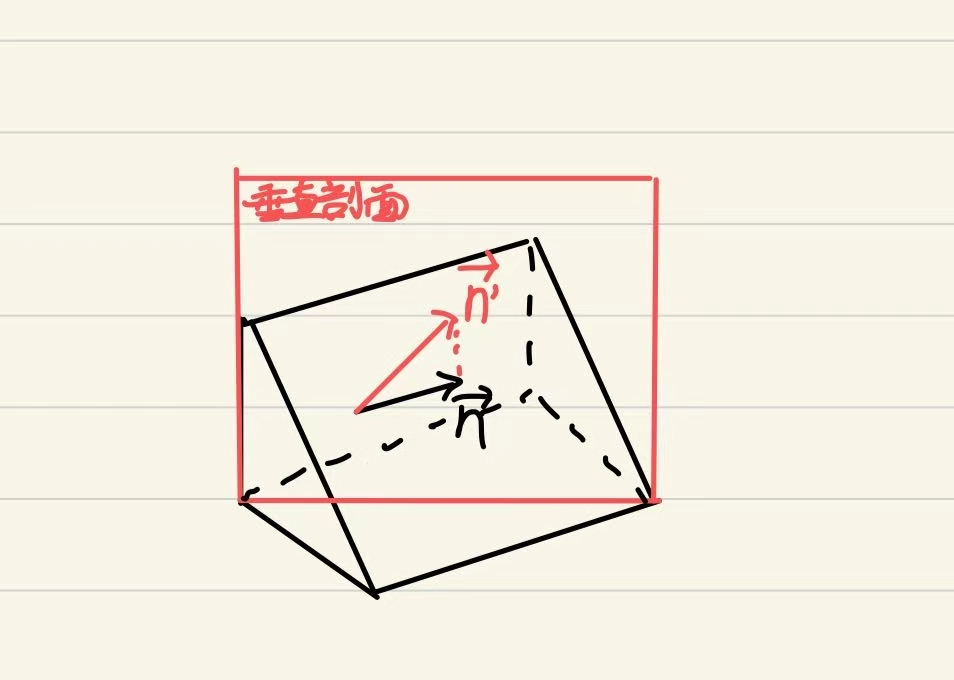
\includegraphics[width=0.6\textwidth]{pic/法线投影.jpg}
      \caption{法线投影}
      \label{fig:法线投影}
    \end{figure}
  \end{itemize}
  
  \item \textbf{交叉现象}
  \begin{itemize}
    \item \textit{正常情况分析}\\
    当对一口井中不同深度点测量的多个地层倾角数据(每个点代表该深度局部地层的真产状)都进行法线投影到同一个垂直剖面方向时,每个点都会在剖面图上得到一条代表其局部视倾角的线段。如果构造形态在垂向上是简单的、一致的(比如一个单斜或简单的圆柱状褶皱),那么这些投影线在剖面图上应该是大致平行的(或不平行但却是连续渐变的),共同勾勒出构造的形态(如一个单斜或者光滑的背斜曲线)。
    
    \item \textit{交叉现象的合并法线问题}\\
    如果构造形态在垂向上发生变化(幅度变陡/变缓,轴线偏移/倾伏),那么不同深度点的局部地层产状(真倾角/倾向)就会发生显著变化。当这些变化较大的产状数据都投影到同一个剖面方向上时,计算出的投影线段的方向和角度也会差异很大。这些线段在剖面图上就可能相交、交叉甚至发散,不再能简单地用一条光滑曲线连接起来。这时需要找到方法来得到光滑曲线,来解决交叉引起的光滑问题。
    
    \begin{figure}[htbp]
      \centering
      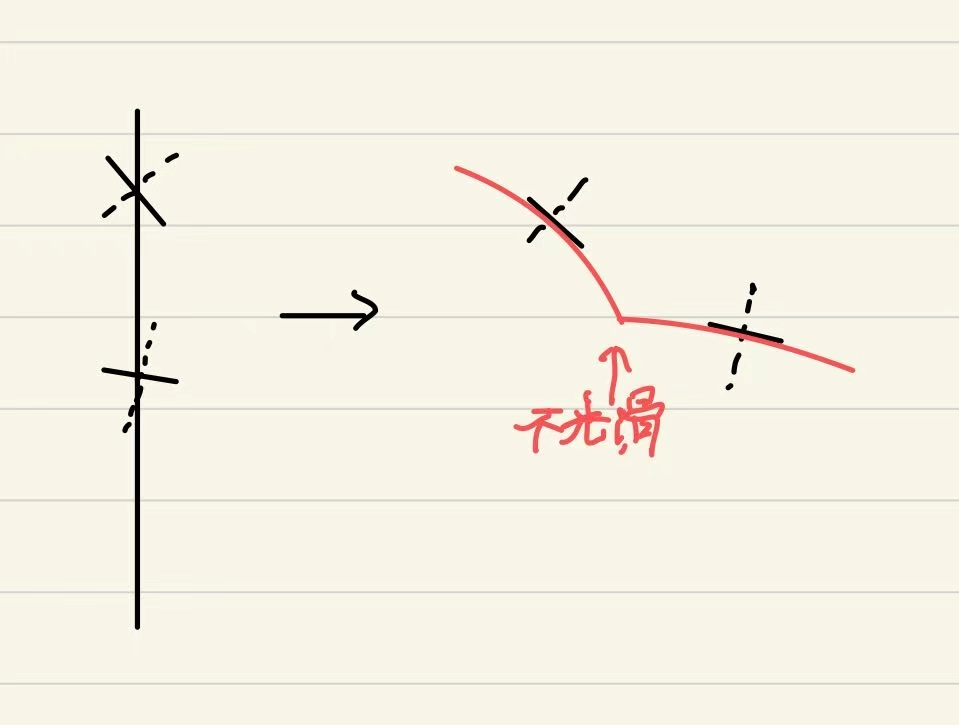
\includegraphics[width=0.6\textwidth]{pic/法线交叉.jpg}
      \caption{法线交叉}
      \label{fig:法线交叉}
    \end{figure}
    
    \begin{figure}[htbp]
      \centering
      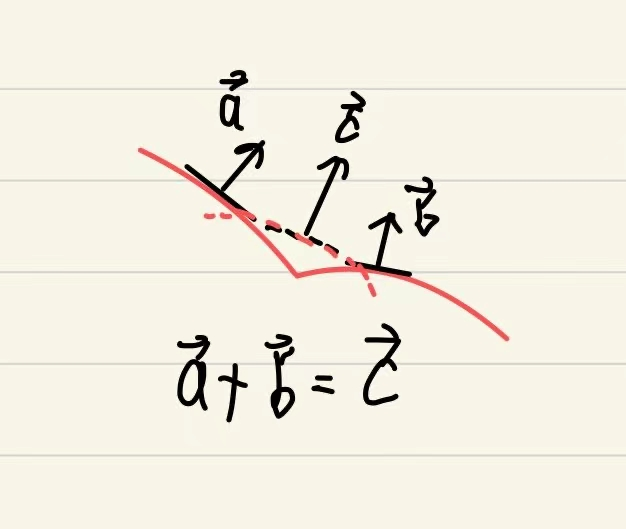
\includegraphics[width=0.6\textwidth]{pic/光滑层线.jpg}
      \caption{光滑层线}
      \label{fig:光滑层线}
    \end{figure}
  \end{itemize}
\end{itemize}

%%%\section{工作量预测}
%%%初步目标为实现二维单斜地质构造剖面生成的程序,初步工作主要分为程序架构设计、核心算法开发以及可视化开发,现阶段预计花费2周时间在程序架构设计,4周时间用于核心算法开发,以及2周时间进行可视化开发,初步开发周期在7-10周左右。
\end{document}
%%% Local Variables:
%%% mode: latex
%%% TeX-master: t
%%% End:
